% SPDX-FileCopyrightText: 2026 Jorge Bernal Martínez
%
% SPDX-License-Identifier: CC-BY-4.0

\documentclass[11pt,a4paper]{article}

\usepackage[T1]{fontenc}
\usepackage[utf8]{inputenc}
\usepackage{lmodern}
\usepackage[english]{babel}
\usepackage[margin=2.5cm]{geometry}
\usepackage{microtype}
\usepackage{amsmath,amssymb}
\usepackage{graphicx}
\usepackage{booktabs}
\usepackage{xcolor}
\usepackage[numbers,sort&compress]{natbib}
\usepackage{caption}
\usepackage{tikz}
\usetikzlibrary{arrows.meta,positioning,fit,calc,backgrounds}
\usepackage[hidelinks]{hyperref}
\usepackage[capitalise,noabbrev]{cleveref}
\usepackage[section]{placeins}

\captionsetup{font=small,labelfont=bf}
\graphicspath{{../figures/en/}}
% Generated by bench/make_tables.py: do not edit.
\newcommand{\nAblHistoryOnlyDeformNat}{-6.87}
\newcommand{\nAblHistoryOnlyDeformNatFlicker}{+101}
\newcommand{\nAblHistoryOnlyDeformQ}{-5.20}
\newcommand{\nAblHistoryOnlyDeformQFlicker}{+81}
\newcommand{\nAblHistoryOnlyFastfloorNat}{-2.57}
\newcommand{\nAblHistoryOnlyFastfloorNatFlicker}{+41}
\newcommand{\nAblHistoryOnlyFastfloorQ}{-1.56}
\newcommand{\nAblHistoryOnlyFastfloorQFlicker}{+29}
\newcommand{\nAblHistoryOnlyFloorNat}{-5.28}
\newcommand{\nAblHistoryOnlyFloorNatFlicker}{+77}
\newcommand{\nAblHistoryOnlyFloorQ}{-4.88}
\newcommand{\nAblHistoryOnlyFloorQFlicker}{+73}
\newcommand{\nAblHistoryOnlyNat}{-5.65}
\newcommand{\nAblHistoryOnlyPanNat}{-6.97}
\newcommand{\nAblHistoryOnlyPanNatFlicker}{+105}
\newcommand{\nAblHistoryOnlyPanQ}{-5.32}
\newcommand{\nAblHistoryOnlyPanQFlicker}{+86}
\newcommand{\nAblHistoryOnlyPausestopNat}{-3.37}
\newcommand{\nAblHistoryOnlyPausestopNatFlicker}{+20}
\newcommand{\nAblHistoryOnlyPausestopQ}{-3.27}
\newcommand{\nAblHistoryOnlyPausestopQFlicker}{+11}
\newcommand{\nAblHistoryOnlyQ}{-4.41}
\newcommand{\nAblHistoryOnlyRest}{3.37}
\newcommand{\nAblHistoryOnlyShadowNat}{-1.20}
\newcommand{\nAblHistoryOnlyShadowNatFlicker}{+34}
\newcommand{\nAblHistoryOnlyShadowQ}{-0.80}
\newcommand{\nAblHistoryOnlyShadowQFlicker}{-39}
\newcommand{\nAblHistoryOnlySmokeNat}{-6.46}
\newcommand{\nAblHistoryOnlySmokeNatFlicker}{+91}
\newcommand{\nAblHistoryOnlySmokeQ}{-4.88}
\newcommand{\nAblHistoryOnlySmokeQFlicker}{+69}
\newcommand{\nAblHistoryOnlyStaticNat}{-0.00}
\newcommand{\nAblHistoryOnlyStaticNatFlicker}{-0}
\newcommand{\nAblHistoryOnlyStaticQ}{-0.00}
\newcommand{\nAblHistoryOnlyStaticQFlicker}{+0}
\newcommand{\nAblHistoryOnlyTgtNat}{+50}
\newcommand{\nAblHistoryOnlyTgtNatAbs}{50}
\newcommand{\nAblHistoryOnlyTgtQ}{+31}
\newcommand{\nAblHistoryOnlyTgtQAbs}{31}
\newcommand{\nAblHistoryOnlyWiresNat}{-5.76}
\newcommand{\nAblHistoryOnlyWiresNatFlicker}{+83}
\newcommand{\nAblHistoryOnlyWiresQ}{-4.62}
\newcommand{\nAblHistoryOnlyWiresQFlicker}{+68}
\newcommand{\nAblNoDeformedWindowDeformNat}{-0.59}
\newcommand{\nAblNoDeformedWindowDeformNatFlicker}{+7}
\newcommand{\nAblNoDeformedWindowDeformQ}{-0.72}
\newcommand{\nAblNoDeformedWindowDeformQFlicker}{+11}
\newcommand{\nAblNoDeformedWindowFastfloorNat}{+0.00}
\newcommand{\nAblNoDeformedWindowFastfloorNatFlicker}{+0}
\newcommand{\nAblNoDeformedWindowFastfloorQ}{+0.00}
\newcommand{\nAblNoDeformedWindowFastfloorQFlicker}{+0}
\newcommand{\nAblNoDeformedWindowFloorNat}{+0.00}
\newcommand{\nAblNoDeformedWindowFloorNatFlicker}{+0}
\newcommand{\nAblNoDeformedWindowFloorQ}{+0.00}
\newcommand{\nAblNoDeformedWindowFloorQFlicker}{+0}
\newcommand{\nAblNoDeformedWindowNat}{-0.59}
\newcommand{\nAblNoDeformedWindowPanNat}{+0.00}
\newcommand{\nAblNoDeformedWindowPanNatFlicker}{+0}
\newcommand{\nAblNoDeformedWindowPanQ}{+0.00}
\newcommand{\nAblNoDeformedWindowPanQFlicker}{+0}
\newcommand{\nAblNoDeformedWindowPausestopNat}{+0.00}
\newcommand{\nAblNoDeformedWindowPausestopNatFlicker}{+0}
\newcommand{\nAblNoDeformedWindowPausestopQ}{+0.00}
\newcommand{\nAblNoDeformedWindowPausestopQFlicker}{+0}
\newcommand{\nAblNoDeformedWindowQ}{-0.72}
\newcommand{\nAblNoDeformedWindowRest}{0.00}
\newcommand{\nAblNoDeformedWindowShadowNat}{+0.00}
\newcommand{\nAblNoDeformedWindowShadowNatFlicker}{+0}
\newcommand{\nAblNoDeformedWindowShadowQ}{+0.00}
\newcommand{\nAblNoDeformedWindowShadowQFlicker}{+0}
\newcommand{\nAblNoDeformedWindowSmokeNat}{+0.00}
\newcommand{\nAblNoDeformedWindowSmokeNatFlicker}{+0}
\newcommand{\nAblNoDeformedWindowSmokeQ}{+0.00}
\newcommand{\nAblNoDeformedWindowSmokeQFlicker}{+0}
\newcommand{\nAblNoDeformedWindowStaticNat}{+0.00}
\newcommand{\nAblNoDeformedWindowStaticNatFlicker}{+0}
\newcommand{\nAblNoDeformedWindowStaticQ}{+0.00}
\newcommand{\nAblNoDeformedWindowStaticQFlicker}{+0}
\newcommand{\nAblNoDeformedWindowTgtNat}{+62}
\newcommand{\nAblNoDeformedWindowTgtNatAbs}{62}
\newcommand{\nAblNoDeformedWindowTgtQ}{+104}
\newcommand{\nAblNoDeformedWindowTgtQAbs}{104}
\newcommand{\nAblNoDeformedWindowWiresNat}{+0.00}
\newcommand{\nAblNoDeformedWindowWiresNatFlicker}{+0}
\newcommand{\nAblNoDeformedWindowWiresQ}{+0.00}
\newcommand{\nAblNoDeformedWindowWiresQFlicker}{+0}
\newcommand{\nAblNoLocksDeformNat}{+0.00}
\newcommand{\nAblNoLocksDeformNatFlicker}{+0}
\newcommand{\nAblNoLocksDeformQ}{+0.00}
\newcommand{\nAblNoLocksDeformQFlicker}{+0}
\newcommand{\nAblNoLocksFastfloorNat}{-0.41}
\newcommand{\nAblNoLocksFastfloorNatFlicker}{+1}
\newcommand{\nAblNoLocksFastfloorQ}{-0.09}
\newcommand{\nAblNoLocksFastfloorQFlicker}{+0}
\newcommand{\nAblNoLocksFloorNat}{-0.88}
\newcommand{\nAblNoLocksFloorNatFlicker}{+1}
\newcommand{\nAblNoLocksFloorQ}{-0.38}
\newcommand{\nAblNoLocksFloorQFlicker}{+1}
\newcommand{\nAblNoLocksNat}{-2.56}
\newcommand{\nAblNoLocksPanNat}{+0.00}
\newcommand{\nAblNoLocksPanNatFlicker}{+0}
\newcommand{\nAblNoLocksPanQ}{+0.00}
\newcommand{\nAblNoLocksPanQFlicker}{+0}
\newcommand{\nAblNoLocksPausestopNat}{-4.86}
\newcommand{\nAblNoLocksPausestopNatFlicker}{+64}
\newcommand{\nAblNoLocksPausestopQ}{-5.05}
\newcommand{\nAblNoLocksPausestopQFlicker}{+160}
\newcommand{\nAblNoLocksQ}{-2.88}
\newcommand{\nAblNoLocksRest}{0.00}
\newcommand{\nAblNoLocksShadowNat}{+0.00}
\newcommand{\nAblNoLocksShadowNatFlicker}{+0}
\newcommand{\nAblNoLocksShadowQ}{+0.00}
\newcommand{\nAblNoLocksShadowQFlicker}{+0}
\newcommand{\nAblNoLocksSmokeNat}{+0.00}
\newcommand{\nAblNoLocksSmokeNatFlicker}{+0}
\newcommand{\nAblNoLocksSmokeQ}{+0.00}
\newcommand{\nAblNoLocksSmokeQFlicker}{+0}
\newcommand{\nAblNoLocksStaticNat}{-4.11}
\newcommand{\nAblNoLocksStaticNatFlicker}{+118}
\newcommand{\nAblNoLocksStaticQ}{-6.01}
\newcommand{\nAblNoLocksStaticQFlicker}{+360}
\newcommand{\nAblNoLocksTgtNat}{+25}
\newcommand{\nAblNoLocksTgtNatAbs}{25}
\newcommand{\nAblNoLocksTgtQ}{+3}
\newcommand{\nAblNoLocksTgtQAbs}{3}
\newcommand{\nAblNoLocksWiresNat}{+0.00}
\newcommand{\nAblNoLocksWiresNatFlicker}{+0}
\newcommand{\nAblNoLocksWiresQ}{+0.00}
\newcommand{\nAblNoLocksWiresQFlicker}{+0}
\newcommand{\nAblNoMissingFillDeformNat}{-0.16}
\newcommand{\nAblNoMissingFillDeformNatFlicker}{+2}
\newcommand{\nAblNoMissingFillDeformQ}{-0.11}
\newcommand{\nAblNoMissingFillDeformQFlicker}{+2}
\newcommand{\nAblNoMissingFillFastfloorNat}{-0.38}
\newcommand{\nAblNoMissingFillFastfloorNatFlicker}{+2}
\newcommand{\nAblNoMissingFillFastfloorQ}{-0.41}
\newcommand{\nAblNoMissingFillFastfloorQFlicker}{+4}
\newcommand{\nAblNoMissingFillFloorNat}{-0.35}
\newcommand{\nAblNoMissingFillFloorNatFlicker}{+3}
\newcommand{\nAblNoMissingFillFloorQ}{-0.45}
\newcommand{\nAblNoMissingFillFloorQFlicker}{+5}
\newcommand{\nAblNoMissingFillNat}{-0.35}
\newcommand{\nAblNoMissingFillPanNat}{-0.19}
\newcommand{\nAblNoMissingFillPanNatFlicker}{+2}
\newcommand{\nAblNoMissingFillPanQ}{-0.14}
\newcommand{\nAblNoMissingFillPanQFlicker}{+2}
\newcommand{\nAblNoMissingFillPausestopNat}{+0.00}
\newcommand{\nAblNoMissingFillPausestopNatFlicker}{+0}
\newcommand{\nAblNoMissingFillPausestopQ}{-0.00}
\newcommand{\nAblNoMissingFillPausestopQFlicker}{+0}
\newcommand{\nAblNoMissingFillQ}{-0.37}
\newcommand{\nAblNoMissingFillRest}{0.01}
\newcommand{\nAblNoMissingFillShadowNat}{+0.00}
\newcommand{\nAblNoMissingFillShadowNatFlicker}{+0}
\newcommand{\nAblNoMissingFillShadowQ}{+0.00}
\newcommand{\nAblNoMissingFillShadowQFlicker}{+0}
\newcommand{\nAblNoMissingFillSmokeNat}{-0.01}
\newcommand{\nAblNoMissingFillSmokeNatFlicker}{+0}
\newcommand{\nAblNoMissingFillSmokeQ}{-0.01}
\newcommand{\nAblNoMissingFillSmokeQFlicker}{+0}
\newcommand{\nAblNoMissingFillStaticNat}{+0.00}
\newcommand{\nAblNoMissingFillStaticNatFlicker}{+0}
\newcommand{\nAblNoMissingFillStaticQ}{+0.00}
\newcommand{\nAblNoMissingFillStaticQFlicker}{+0}
\newcommand{\nAblNoMissingFillTgtNat}{+27}
\newcommand{\nAblNoMissingFillTgtNatAbs}{27}
\newcommand{\nAblNoMissingFillTgtQ}{+25}
\newcommand{\nAblNoMissingFillTgtQAbs}{25}
\newcommand{\nAblNoMissingFillWiresNat}{-0.65}
\newcommand{\nAblNoMissingFillWiresNatFlicker}{+4}
\newcommand{\nAblNoMissingFillWiresQ}{-0.74}
\newcommand{\nAblNoMissingFillWiresQFlicker}{+8}
\newcommand{\nAblNoReactiveNat}{-2.27}
\newcommand{\nAblNoReactiveQ}{-1.44}
\newcommand{\nAblNoReactiveRest}{0.00}
\newcommand{\nAblNoReactiveSmokeNat}{-2.27}
\newcommand{\nAblNoReactiveSmokeNatFlicker}{+4}
\newcommand{\nAblNoReactiveSmokeQ}{-1.44}
\newcommand{\nAblNoReactiveSmokeQFlicker}{+1}
\newcommand{\nAblNoReactiveTgtNat}{+133}
\newcommand{\nAblNoReactiveTgtNatAbs}{133}
\newcommand{\nAblNoReactiveTgtQ}{+140}
\newcommand{\nAblNoReactiveTgtQAbs}{140}
\newcommand{\nAblNoThinFrontDeformNat}{+0.00}
\newcommand{\nAblNoThinFrontDeformNatFlicker}{+0}
\newcommand{\nAblNoThinFrontDeformQ}{+0.00}
\newcommand{\nAblNoThinFrontDeformQFlicker}{+0}
\newcommand{\nAblNoThinFrontFastfloorNat}{+0.00}
\newcommand{\nAblNoThinFrontFastfloorNatFlicker}{+0}
\newcommand{\nAblNoThinFrontFastfloorQ}{+0.00}
\newcommand{\nAblNoThinFrontFastfloorQFlicker}{+0}
\newcommand{\nAblNoThinFrontFloorNat}{+0.00}
\newcommand{\nAblNoThinFrontFloorNatFlicker}{+0}
\newcommand{\nAblNoThinFrontFloorQ}{+0.00}
\newcommand{\nAblNoThinFrontFloorQFlicker}{+0}
\newcommand{\nAblNoThinFrontNat}{-0.22}
\newcommand{\nAblNoThinFrontPanNat}{+0.00}
\newcommand{\nAblNoThinFrontPanNatFlicker}{+0}
\newcommand{\nAblNoThinFrontPanQ}{+0.00}
\newcommand{\nAblNoThinFrontPanQFlicker}{+0}
\newcommand{\nAblNoThinFrontPausestopNat}{+0.00}
\newcommand{\nAblNoThinFrontPausestopNatFlicker}{-0}
\newcommand{\nAblNoThinFrontPausestopQ}{+0.00}
\newcommand{\nAblNoThinFrontPausestopQFlicker}{-0}
\newcommand{\nAblNoThinFrontQ}{-0.16}
\newcommand{\nAblNoThinFrontRest}{0.00}
\newcommand{\nAblNoThinFrontShadowNat}{+0.00}
\newcommand{\nAblNoThinFrontShadowNatFlicker}{+0}
\newcommand{\nAblNoThinFrontShadowQ}{+0.00}
\newcommand{\nAblNoThinFrontShadowQFlicker}{+0}
\newcommand{\nAblNoThinFrontSmokeNat}{-0.00}
\newcommand{\nAblNoThinFrontSmokeNatFlicker}{-0}
\newcommand{\nAblNoThinFrontSmokeQ}{-0.00}
\newcommand{\nAblNoThinFrontSmokeQFlicker}{+0}
\newcommand{\nAblNoThinFrontStaticNat}{+0.00}
\newcommand{\nAblNoThinFrontStaticNatFlicker}{+0}
\newcommand{\nAblNoThinFrontStaticQ}{+0.00}
\newcommand{\nAblNoThinFrontStaticQFlicker}{+0}
\newcommand{\nAblNoThinFrontTgtNat}{+12}
\newcommand{\nAblNoThinFrontTgtNatAbs}{12}
\newcommand{\nAblNoThinFrontTgtQ}{+12}
\newcommand{\nAblNoThinFrontTgtQAbs}{12}
\newcommand{\nAblNoThinFrontWiresNat}{-0.22}
\newcommand{\nAblNoThinFrontWiresNatFlicker}{+3}
\newcommand{\nAblNoThinFrontWiresQ}{-0.16}
\newcommand{\nAblNoThinFrontWiresQFlicker}{+0}
\newcommand{\nAblWindowOnlyDeformNat}{+0.00}
\newcommand{\nAblWindowOnlyDeformNatFlicker}{+0}
\newcommand{\nAblWindowOnlyDeformQ}{+0.00}
\newcommand{\nAblWindowOnlyDeformQFlicker}{+0}
\newcommand{\nAblWindowOnlyFastfloorNat}{+0.02}
\newcommand{\nAblWindowOnlyFastfloorNatFlicker}{-0}
\newcommand{\nAblWindowOnlyFastfloorQ}{+0.00}
\newcommand{\nAblWindowOnlyFastfloorQFlicker}{+0}
\newcommand{\nAblWindowOnlyFloorNat}{+0.03}
\newcommand{\nAblWindowOnlyFloorNatFlicker}{-1}
\newcommand{\nAblWindowOnlyFloorQ}{-0.01}
\newcommand{\nAblWindowOnlyFloorQFlicker}{-0}
\newcommand{\nAblWindowOnlyNat}{-0.30}
\newcommand{\nAblWindowOnlyPanNat}{+0.00}
\newcommand{\nAblWindowOnlyPanNatFlicker}{+0}
\newcommand{\nAblWindowOnlyPanQ}{+0.00}
\newcommand{\nAblWindowOnlyPanQFlicker}{+0}
\newcommand{\nAblWindowOnlyPausestopNat}{+0.38}
\newcommand{\nAblWindowOnlyPausestopNatFlicker}{+58}
\newcommand{\nAblWindowOnlyPausestopQ}{+0.33}
\newcommand{\nAblWindowOnlyPausestopQFlicker}{+38}
\newcommand{\nAblWindowOnlyQ}{-0.03}
\newcommand{\nAblWindowOnlyRest}{0.03}
\newcommand{\nAblWindowOnlyShadowNat}{+0.00}
\newcommand{\nAblWindowOnlyShadowNatFlicker}{+0}
\newcommand{\nAblWindowOnlyShadowQ}{+0.00}
\newcommand{\nAblWindowOnlyShadowQFlicker}{+0}
\newcommand{\nAblWindowOnlySmokeNat}{+0.00}
\newcommand{\nAblWindowOnlySmokeNatFlicker}{+0}
\newcommand{\nAblWindowOnlySmokeQ}{+0.00}
\newcommand{\nAblWindowOnlySmokeQFlicker}{+0}
\newcommand{\nAblWindowOnlyStaticNat}{-0.97}
\newcommand{\nAblWindowOnlyStaticNatFlicker}{+161}
\newcommand{\nAblWindowOnlyStaticQ}{-0.39}
\newcommand{\nAblWindowOnlyStaticQFlicker}{+147}
\newcommand{\nAblWindowOnlyTgtNat}{+161}
\newcommand{\nAblWindowOnlyTgtNatAbs}{161}
\newcommand{\nAblWindowOnlyTgtQ}{+147}
\newcommand{\nAblWindowOnlyTgtQAbs}{147}
\newcommand{\nAblWindowOnlyWiresNat}{+0.00}
\newcommand{\nAblWindowOnlyWiresNatFlicker}{+0}
\newcommand{\nAblWindowOnlyWiresQ}{+0.00}
\newcommand{\nAblWindowOnlyWiresQFlicker}{+0}
\newcommand{\nFlickerB}{11.1}
\newcommand{\nFlickerNat}{7.1}
\newcommand{\nFlickerNoAA}{24.3}
\newcommand{\nFlickerP}{12.0}
\newcommand{\nFlickerQ}{9.8}
\newcommand{\nFlickerTAAg}{12.8}
\newcommand{\nFlickerTAApt}{11.9}
\newcommand{\nFlickerUQ}{8.8}
\newcommand{\nFlipB}{0.0398}
\newcommand{\nFlipNat}{0.0236}
\newcommand{\nFlipNoAA}{0.0467}
\newcommand{\nFlipP}{0.0419}
\newcommand{\nFlipQ}{0.0340}
\newcommand{\nFlipTAAg}{0.0409}
\newcommand{\nFlipTAApt}{0.0487}
\newcommand{\nFlipUQ}{0.0309}
\newcommand{\nGainAllB}{1.78}
\newcommand{\nGainAllNat}{5.75}
\newcommand{\nGainAllP}{1.00}
\newcommand{\nGainAllQ}{2.84}
\newcommand{\nGainAllUQ}{3.92}
\newcommand{\nGainMotionB}{1.53}
\newcommand{\nGainMotionNat}{5.85}
\newcommand{\nGainMotionP}{0.69}
\newcommand{\nGainMotionQ}{2.82}
\newcommand{\nGainMotionUQ}{3.87}
\newcommand{\nGhostCutNat}{49}
\newcommand{\nGhostCutP}{49}
\newcommand{\nGhostCutQ}{47}
\newcommand{\nGhostHistNatOne}{23.0}
\newcommand{\nGhostHistPOne}{34.0}
\newcommand{\nGhostHistQOne}{28.2}
\newcommand{\nGhostHwNatOne}{18.1}
\newcommand{\nGhostHwPOne}{30.7}
\newcommand{\nGhostHwQOne}{26.6}
\newcommand{\nGhostNoFillNatOne}{35.3}
\newcommand{\nGhostNoFillPOne}{59.9}
\newcommand{\nGhostNoFillQOne}{49.8}
\newcommand{\nGhostTaaNatOne}{32.2}
\newcommand{\nGhostVsHistNat}{44}
\newcommand{\nGhostVsHistP}{29}
\newcommand{\nGhostVsHistQ}{35}
\newcommand{\nHistShareB}{29}
\newcommand{\nHistShareNat}{47}
\newcommand{\nHistShareP}{33}
\newcommand{\nHistShareQ}{29}
\newcommand{\nHistShareUQ}{29}
\newcommand{\nMemBHd}{127}
\newcommand{\nMemBQhd}{226}
\newcommand{\nMemBUhd}{508}
\newcommand{\nMemNatHd}{189}
\newcommand{\nMemNatQhd}{335}
\newcommand{\nMemNatUhd}{755}
\newcommand{\nMemPHd}{95}
\newcommand{\nMemPQhd}{169}
\newcommand{\nMemPUhd}{379}
\newcommand{\nMemQHd}{151}
\newcommand{\nMemQQhd}{269}
\newcommand{\nMemQUhd}{605}
\newcommand{\nMemUQHd}{188}
\newcommand{\nMemUQQhd}{333}
\newcommand{\nMemUQUhd}{750}
\newcommand{\nMsMovingBHd}{2.0}
\newcommand{\nMsMovingBQhd}{3.6}
\newcommand{\nMsMovingBUhd}{8.0}
\newcommand{\nMsMovingNatHd}{1.4}
\newcommand{\nMsMovingNatQhd}{2.5}
\newcommand{\nMsMovingNatUhd}{5.5}
\newcommand{\nMsMovingPHd}{1.8}
\newcommand{\nMsMovingPQhd}{3.1}
\newcommand{\nMsMovingPUhd}{7.0}
\newcommand{\nMsMovingQHd}{2.0}
\newcommand{\nMsMovingQQhd}{3.6}
\newcommand{\nMsMovingQUhd}{8.1}
\newcommand{\nMsMovingUQHd}{2.0}
\newcommand{\nMsMovingUQQhd}{3.6}
\newcommand{\nMsMovingUQUhd}{8.2}
\newcommand{\nMsPerFrameHd}{0.12}
\newcommand{\nMsPerFrameUhd}{0.48}
\newcommand{\nMsStillBHd}{0.6}
\newcommand{\nMsStillBQhd}{1.1}
\newcommand{\nMsStillBUhd}{2.5}
\newcommand{\nMsStillNatHd}{0.8}
\newcommand{\nMsStillNatQhd}{1.4}
\newcommand{\nMsStillNatUhd}{3.2}
\newcommand{\nMsStillPHd}{0.6}
\newcommand{\nMsStillPQhd}{1.1}
\newcommand{\nMsStillPUhd}{2.4}
\newcommand{\nMsStillQHd}{0.6}
\newcommand{\nMsStillQQhd}{1.1}
\newcommand{\nMsStillQUhd}{2.6}
\newcommand{\nMsStillUQHd}{0.7}
\newcommand{\nMsStillUQQhd}{1.2}
\newcommand{\nMsStillUQUhd}{2.6}
\newcommand{\nNumScenes}{13}
\newcommand{\nPsnrAllB}{31.85}
\newcommand{\nPsnrAllBestTAA}{30.06}
\newcommand{\nPsnrAllNat}{35.81}
\newcommand{\nPsnrAllNoAA}{27.62}
\newcommand{\nPsnrAllP}{31.07}
\newcommand{\nPsnrAllQ}{32.90}
\newcommand{\nPsnrAllTAAg}{29.45}
\newcommand{\nPsnrAllTAApt}{30.04}
\newcommand{\nPsnrAllUQ}{33.98}
\newcommand{\nPsnrMotionB}{31.25}
\newcommand{\nPsnrMotionNat}{35.56}
\newcommand{\nPsnrMotionNoAA}{27.14}
\newcommand{\nPsnrMotionP}{30.40}
\newcommand{\nPsnrMotionQ}{32.54}
\newcommand{\nPsnrMotionTAAg}{29.38}
\newcommand{\nPsnrMotionTAApt}{29.68}
\newcommand{\nPsnrMotionUQ}{33.58}
\newcommand{\nWinsB}{12}
\newcommand{\nWinsNat}{13}
\newcommand{\nWinsP}{10}
\newcommand{\nWinsQ}{13}
\newcommand{\nWinsUQ}{13}
\newcommand{\nWorstGainB}{-0.14}
\newcommand{\nWorstGainNat}{3.99}
\newcommand{\nWorstGainP}{-1.10}
\newcommand{\nWorstGainQ}{0.70}
\newcommand{\nWorstGainUQ}{1.57}
\newcommand{\nWorstSceneB}{fast floor}
\newcommand{\nWorstSceneEsB}{suelo r\'apido}
\newcommand{\nWorstSceneEsNat}{suelo r\'apido}
\newcommand{\nWorstSceneEsP}{suelo r\'apido}
\newcommand{\nWorstSceneEsQ}{suelo r\'apido}
\newcommand{\nWorstSceneEsUQ}{suelo r\'apido}
\newcommand{\nWorstSceneNat}{fast floor}
\newcommand{\nWorstSceneP}{fast floor}
\newcommand{\nWorstSceneQ}{fast floor}
\newcommand{\nWorstSceneUQ}{fast floor}

\newcommand{\FLIP}{\reflectbox{F}LIP}
\newcommand{\vect}[1]{\mathbf{#1}}

\title{Hybrid Windowed Temporal Antialiasing:\\Reconstructing Moving Pixels from a Ring of Raw Jittered Samples}
\author{Jorge Bernal Mart\'{\i}nez\\
  \small UPBGE Game Engine developer\\
  \small\texttt{jbernalmartinez@gmail.com}}
\date{November 2026\\[4pt]\footnotesize \copyright{} 2026 Jorge Bernal Mart\'{\i}nez. \\ This work is licensed under the Creative Commons Attribution 4.0 International License (CC BY 4.0).}

\begin{document}
\maketitle

\begin{abstract}
Temporal antialiasing (TAA), and the temporal upscalers built on it, accumulate a recursive history that is resampled every frame a pixel moves. The repeated resampling blurs moving content, and the neighborhood color clamp that limits ghosting also erases thin features. We present \emph{Hybrid Windowed Temporal Antialiasing} (HWTAA). HWTAA keeps the raw jittered samples of the last $N$ frames in a compact ring buffer, 8 bytes per sample, and reconstructs each moving pixel directly from them: every past sample is moved to the current frame once and exactly, through one closed-form matrix per frame, weighted by its distance to the pixel center, and accepted by object identity instead of a color clamp. Pixels at rest keep a recursive history, which converges beyond the window, costs less and flickers less; the two estimators are mixed per pixel by its motion. A missing-weight fill restores the surfaces that moving objects uncover, a reactive mask handles transparent surfaces, and luma locks keep thin features in the history. On \nNumScenes{} synthetic scenes, rendered with the production shaders and compared against a 36-sample reference, HWTAA at native resolution improves PSNR over a production-grade TAA by \nGainAllNat{}\,dB on average and in \nWinsNat{} of \nNumScenes{} scenes; its Quality upscaling mode, which renders 44\,\% of the pixels, still improves it by \nGainAllQ{}\,dB in \nWinsQ{} of \nNumScenes{}. The resolve fits in 64 registers. Its estimated cost at 1080p on a GPU of the GTX~1060 class is \nMsStillQHd{}\,ms for pixels at rest and \nMsMovingQHd{}\,ms with the whole screen in motion (Quality mode). HWTAA ships in the eevee-game renderer of the UPBGE game engine.
\end{abstract}

\section{Introduction}

Real-time renderers take one sample per pixel and per frame and rely on time to supply the rest. Temporal antialiasing~\cite{karis2014taa,salvi2016taa,yang2020survey} jitters the projection by a sub-pixel offset every frame, reprojects an accumulated history to the current frame with motion vectors, rejects the parts of it that no longer belong to the pixel, usually by clamping it to the color range of the current $3\times3$ neighborhood, and blends the current frame in with a small weight. Temporal upscalers such as FSR~2 and 3~\cite{amd2023fsr2,amd2024fsr3}, DLSS~\cite{liu2020dlss} or neural supersampling~\cite{xiao2020neural} extend the same recursion to render resolutions below the output.

The recursion is an infinite impulse response (IIR) filter, and it has two well known weaknesses. First, the history is resampled every frame the pixel moves. Any resampling filter attenuates the frequencies near the pixel Nyquist limit; applied once per frame, the attenuation compounds, and moving content ends up blurred. Yang et al.~\cite{yang2009amortized} analysed this effect and limited it with sub-pixel history buffers and an adaptive blend factor; production TAA reduces it with sharper filters such as Catmull-Rom~\cite{catmull1974splines,jimenez2016filmic}. Second, the color clamp cannot tell an undersampled thin feature from a disoccluded one: a cable one tenth of a pixel wide is absent from most current neighborhoods, so the clamp erases what the history had accumulated, and the result flickers.

We observe that the information TAA needs is already computed every frame: it is the jittered samples themselves. A history is a lossy summary of them, convenient because it costs one texture per frame. If the raw samples of a short window of frames are kept instead, a moving pixel can be reconstructed from them directly. Each past sample is then moved to the current frame exactly once, from its own depth and the camera and object transforms of both frames, so no intermediate image is ever resampled. Visibility can be decided by the identity of the surface a sample belongs to, which is exact, instead of by color statistics, which are not. This is a finite impulse response (FIR) estimator. Its weakness is the converse of the history's: its support is $N$ frames, so a pixel at rest converges no further than $N$ samples, while a history converges indefinitely and costs a few taps.

HWTAA combines both. Moving pixels use the window, pixels at rest use the history, and the output mixes them by the pixel's motion. Our contributions are:
\begin{itemize}
\item A hybrid FIR/IIR temporal estimator selected per pixel by motion, in which the window removes the resampling blur of moving content and the history keeps the convergence, stability and low cost of TAA for content at rest (\cref{sec:overview}).
\item A sample ring that stores, per render texel and frame, the object key, inverse depth, stability and transparency flags, color and median luma in 8 bytes (\cref{sec:ring}).
\item A closed-form per-sample reprojection: one $4\times4$ matrix per past frame maps a render texel and its inverse depth directly to the weight space of the output pixel, so a sample costs three multiply-adds, one division and one shared-memory read (\cref{sec:window}).
\item Visibility by identity without color clamping, a missing-weight fill for disoccluded surfaces, and frame rejection by median luma for shading that moves on its own (\cref{sec:window,sec:missing,sec:reactive}).
\item An evaluation on \nNumScenes{} scenes that runs the production GLSL shaders, with PSNR, \FLIP{}~\cite{andersson2020flip}, SSIM~\cite{wang2004ssim} and a flicker metric, ablations of every component, and a cost and memory model checked against AMD's published FSR figures (\cref{sec:evaluation}).
\end{itemize}

\section{Related work}

\paragraph{Spatial antialiasing.} Morphological filters such as FXAA~\cite{lottes2009fxaa} and SMAA~\cite{jimenez2012smaa} detect edges in the final image and blend across them. They are cheap and stable but cannot recover detail that the single sample per pixel missed, which is the case of thin features and sub-pixel texture.

\paragraph{Reprojection and amortized supersampling.} Reverse reprojection caching~\cite{nehab2007reprojection} reuses shading from the previous frame by projecting the current pixel into it. Amortized supersampling~\cite{yang2009amortized} accumulates jittered samples recursively, analyses the blur caused by resampling the history and reduces it with several sub-pixel buffers. Spatio-temporal upsampling~\cite{herzog2010upsampling} combines a recursive temporal filter with a joint bilateral spatial filter. Scherzer et al.~\cite{scherzer2012coherence} survey these methods. All of them keep a recursive history; HWTAA keeps one too, for pixels at rest, and replaces it for moving pixels.

\paragraph{Temporal antialiasing and upscaling in games.} TAA as used in games~\cite{karis2014taa,jimenez2016filmic} reprojects a history with motion vectors, samples it with a sharp filter and clamps or clips it to the current neighborhood; variance clipping~\cite{salvi2016taa} fits the clip box to the neighborhood's mean and standard deviation. Yang et al.~\cite{yang2020survey} survey the family and its artifacts: blur, ghosting, flicker and loss of thin features. Adaptive TAA~\cite{marrs2018ataa} ray traces the pixels where the history fails. FSR~2~\cite{amd2023fsr2} adds depth-based disocclusion detection, a reactive mask for transparent surfaces and \emph{locks} that protect thin features from the clamp; HWTAA's history uses locks with the same purpose and a different detection and lifetime (\cref{sec:history}). Learned upscalers~\cite{liu2020dlss,xiao2020neural} replace the hand-made rejection by a network, but still feed it a warped history. Poudel et al.~\cite{poudel2026wavelet} split a neural upscaler's output into frequency bands; a split of the history into a low band that is clipped and a high band that is kept is used here for pixels at rest when upscaling.

\paragraph{Frameless rendering and deep sample buffers.} Frameless rendering~\cite{bishop1994frameless} updates samples asynchronously and displays whatever the buffer holds; the render cache~\cite{walter1999rendercache} reprojects individual ray-traced samples to new views as points. Adaptive frameless rendering~\cite{dayal2005frameless} is the closest prior work: it keeps the recent samples of a frameless ray tracer in a \emph{temporally deep buffer} and reconstructs each displayed image with space-time filters whose extent adapts to the local spatial and temporal change. HWTAA differs from it in three ways. Each past sample is moved to the current frame with exact geometry, which removes motion from the filter instead of narrowing it. Visibility is decided by object identity. And the window is one half of a hybrid with a recursive history, at a fixed cost per frame inside a rasterization pipeline. We are not aware of a real-time TAA or temporal upscaler that reconstructs moving pixels from a window of raw past samples reprojected individually.

\paragraph{Denoising.} Spatio-temporal variance-guided filtering~\cite{schied2017svgf} and its successors also accumulate a history validated by depth, normals and object identity. Our identity test is of the same nature; the difference is again that the window does not accumulate.

\section{Method}
\label{sec:method}

\subsection{Overview}
\label{sec:overview}

\begin{figure}[t]
\centering
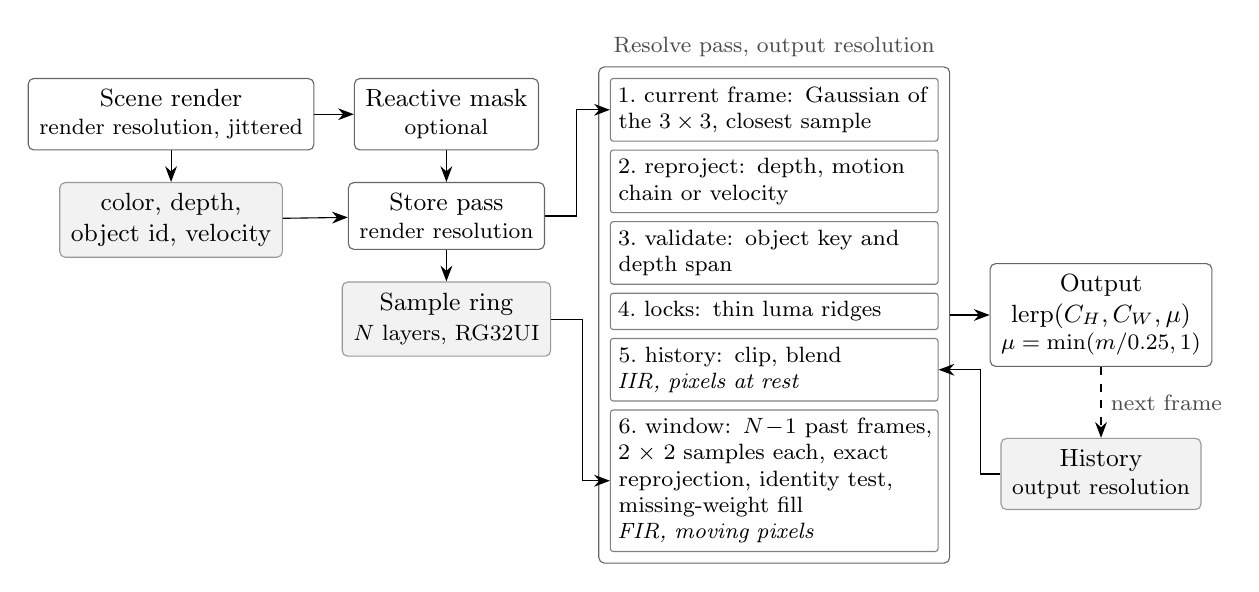
\begin{tikzpicture}[
  font=\small, >={Stealth[length=2mm]},
  box/.style={draw=black!60, rounded corners=2pt, align=center, inner sep=4pt, fill=white},
  data/.style={draw=black!40, fill=black!5, rounded corners=2pt, align=center, inner sep=4pt},
  stage/.style={draw=black!50, rounded corners=1pt, align=left, inner sep=3pt, fill=white, font=\footnotesize, text width=3.95cm},
  lbl/.style={font=\footnotesize, text=black!70}]
\node[box] (render) {Scene render\\[-1pt]{\footnotesize render resolution, jittered}};
\node[data, below=4mm of render] (gbuf) {color, depth,\\object id, velocity};
\node[box, right=5mm of render] (react) {Reactive mask\\[-1pt]{\footnotesize optional}};
\node[box, below=4mm of react] (store) {Store pass\\[-1pt]{\footnotesize render resolution}};
\node[data, below=4mm of store] (ring) {Sample ring\\{\footnotesize $N$ layers, RG32UI}};
\node[stage, right=9mm of react.north east, anchor=north west] (s1) {1.\ current frame: Gaussian of the $3\times3$, closest sample};
\node[stage, below=1mm of s1] (s2) {2.\ reproject: depth, motion chain or velocity};
\node[stage, below=1mm of s2] (s3) {3.\ validate: object key and depth span};
\node[stage, below=1mm of s3] (s4) {4.\ locks: thin luma ridges};
\node[stage, below=1mm of s4] (s5) {5.\ history: clip, blend\\\textit{IIR, pixels at rest}};
\node[stage, below=1mm of s5] (s6) {6.\ window: $N\!-\!1$ past frames, $2\times2$ samples each, exact reprojection, identity test, missing-weight fill\\\textit{FIR, moving pixels}};
\node[draw=black!60, rounded corners=2pt, inner sep=4pt, fit=(s1)(s6)] (resolve) {};
\node[lbl, above=0mm of resolve.north] {Resolve pass, output resolution};
\node[box, right=5mm of resolve] (out) {Output\\$\mathrm{lerp}(C_H, C_W, \mu)$\\[-1pt]{\footnotesize $\mu=\min(m/0.25,1)$}};
\node[data, below=9mm of out] (hist) {History\\[-1pt]{\footnotesize output resolution}};
\draw[->] (render) -- (react);
\draw[->] (render) -- (gbuf);
\draw[->] (react) -- (store);
\draw[->] (gbuf) -- (store);
\draw[->] (store) -- (ring);
\draw[->] (ring.east) -- ++(4mm,0) |- (s6.west);
\draw[->] (store.east) -- ++(4mm,0) |- (s1.west);
\draw[->] (resolve) -- (out);
\draw[->, dashed] (out) -- node[lbl, right] {next frame} (hist);
\draw[->] (hist.west) -- ++(-2.5mm,0) |- (s5.east);
\end{tikzpicture}
\caption{HWTAA per frame. The store pass writes the frame's samples into one layer of the ring. The resolve runs once per output pixel: steps 1 to 4 run for every pixel, step 5 for pixels that move less than $0.25$ output pixels per frame, step 6 for pixels that move more than zero, and the output mixes the history $C_H$ and the window $C_W$ by the motion $m$.}
\label{fig:pipeline}
\end{figure}

HWTAA runs as two compute passes after the opaque and transparent geometry (\cref{fig:pipeline}). The renderer provides, at render resolution and with a Halton$(2,3)$~\cite{halton1964} jitter: linear HDR color, depth, a per-pixel resource identifier that maps to a stable object key and to the object's motion, and a velocity buffer for deformed meshes. The \emph{store pass} packs the frame's samples into one layer of a ring buffer of $N$ layers. The \emph{resolve pass} reconstructs every output pixel. It always reconstructs the current frame at the pixel center and reprojects and validates the pixel's history. For a pixel at rest it clips and blends the history as TAA does (\cref{sec:history}). For a moving pixel it gathers the samples of the $N-1$ previous frames from the ring (\cref{sec:window}). The output is
\begin{equation}
C = (1-\mu)\, C_H + \mu\, C_W, \qquad \mu = \min\!\left(\frac{m}{m_0}, 1\right), \quad m_0 = 0.25,
\label{eq:mix}
\end{equation}
where $m$ is the motion of the pixel's closest surface in output pixels per frame, $C_H$ the history estimate and $C_W$ the window estimate. Pixels with $\mu = 1$ skip the history sampling, clip and blend; pixels with $\mu=0$ skip the window. The output is written back as the history.

\subsection{Sample ring}
\label{sec:ring}

Each ring texel holds one render sample in two 32-bit words. The \emph{info word} holds a 16-bit object key (0 is the background) and the half-float bits of the inverse view depth $z = 1/d$. The sign bit of the half float, always positive, flags samples of objects that are not static, and its lowest mantissa bit, a 0.1\,\% change of $z$, flags samples covered by transparent surfaces. The \emph{color word} holds the color tone mapped by $c/(1+\max(c))$, square-root encoded in 8 bits per channel, and the median of the tone-mapped luma of the sample's $3\times3$ neighborhood, also in 8 bits. On our scenes this layout matched a 16-bit float color within 0.02\,dB, while 6-bit channels lost 0.2 to 0.3\,dB. Inverse depth is stored because NDC depth is affine in it under perspective projection, which makes the reprojection of \cref{sec:window} a single matrix product, and because the background at infinity is simply $z=0$.

The ring costs $8N$ bytes per render texel. Its length per mode and its memory are given in \cref{sec:cost}; when the GPU memory budget does not hold $N$ layers, the window is shortened, and below 4 layers it is disabled and the method falls back to its history.

\subsection{Current frame and reprojection}
\label{sec:current}

The current frame is reconstructed at the output pixel center $\vect p$ from the $3\times3$ render samples around it:
\begin{equation}
C_0(\vect p) = \frac{\sum_i w_i\, c_i}{\sum_i w_i}, \qquad w_i = e^{-k\,\|\vect x_i - \vect p\|^2}, \quad k = 4,
\label{eq:current}
\end{equation}
where $\vect x_i$ is the jittered position of sample $i$ in output pixels. The largest weight $w_{\max}$ measures how well this frame covers the pixel and is its share in the history blend. The sample with the largest inverse depth in the $3\times3$, the closest one, represents the pixel in the reprojection, so silhouettes follow the foreground. Its world position is moved to the previous frame by the camera alone for static objects, by the object's motion chain (the product of its object-to-world transforms of both frames) for rigidly moving objects, and by the velocity buffer for deformed meshes. The resolve and store passes work on $8\times8$ pixel groups that load the render texels they need once into shared memory.

\subsection{History path}
\label{sec:history}

For pixels at rest HWTAA is a TAA with three changes to the usual design.

\paragraph{Validation by identity.} Instead of detecting disocclusion by color, the history is valid when the $2\times2$ previous samples around the reprojected position, read from the previous ring layer, contain the pixel's object key and the expected inverse depth lies within their depth span (2\,\% slack). A static surface in front of all of them is also valid: it could not have been hidden, the previous samples just missed it, as happens with cables and stochastic transparency.

\paragraph{Clip and confidence.} The history, sampled with a five-tap Catmull-Rom filter~\cite{jimenez2016filmic}, is clipped toward the mean of the variance box~\cite{salvi2016taa} of the $3\times3$ in tone-mapped YCoCg. The box half-size is one standard deviation, or $0.75$ for objects flagged as having volatile shading. A clipped history loses confidence by the square of the clip ratio. The history alpha channel stores its confidence $n$, a sum of sample weights, and the blend is
\begin{equation}
n' = \min(n + w_{\max},\; n_{\max}(m)), \qquad C_H = \mathrm{lerp}(H, C_0, w_{\max}/n'),
\end{equation}
with $n_{\max}(m) = \max(n_{\max}/(1+0.5\,m), 1)$: each resampling blurs the history, so its confidence is capped as the pixel moves. $n_{\max}$ is $8\,s^{-2}$, clamped to $[8,32]$, for a render scale $s$, and 256 when the scene is idle (nothing moved); the jitter cycle is $8\,s^{-2}$ phases in general and 64 when idle, so a still image keeps converging. Averages are taken in linear color, which is the space of the reference, and blends move toward the tone-mapped space as the pixel moves, where isolated bright samples would otherwise smear.

\paragraph{Locks.} A thin feature is a luma ridge (all the neighbors that differ by more than 5\,\% from the center lie on one side of it) that no $2\times2$ quad containing the center explains. Where one is found, a lock is created; while it lives, the history is not clipped. A lock dies when the median luma of the $3\times3$ changes by more than a factor 1.25 from its value at creation, which is insensitive to the feature itself (at most three of nine samples) and follows any shading change that covers the neighborhood, such as a moving shadow. No lock lives on a geometric edge, defined as a $3\times3$ whose inverse depths span more than 2\,\%; the background alone is not an edge, so stars keep their locks. Locks are evaluated for every pixel, including moving ones, so they survive the motion and are ready when the pixel stops.

\paragraph{Frequency split.} When the render scale is at most 0.6 and the scene is idle, the box of the render-resolution $3\times3$ cannot validate frequencies above the render Nyquist limit, and clipping the whole history removes the detail that accumulated beyond it. The history is then split into a low band, the mean of four bilinear taps on the diagonals, $0.5\,(s^{-1}-1)$ output pixels away per axis, which is clipped, and a high band, which is kept within two box half-widths. This gained 0.59\,dB on a static scene at half resolution.

\subsection{Sample window}
\label{sec:window}

For a moving pixel, the window estimate is
\begin{equation}
C_W(\vect p) = \frac{\frac{1}{1-r}\sum_{i} w_i c_i \;+\; \sum_{k=1}^{N-1} \sum_{j\in S_k} v_j\, \omega_j\, c_j \;+\; \omega_{\mathrm{miss}}\, \bar c_{\mathrm{other}}}{\frac{1}{1-r}\sum_i w_i \;+\; \sum_{k=1}^{N-1}\sum_{j\in S_k} v_j\, \omega_j \;+\; \omega_{\mathrm{miss}}},
\label{eq:window}
\end{equation}
where the first terms are the current $3\times3$ of \cref{eq:current}, $S_k$ are the four ring samples of frame $t-k$ nearest to where the pixel's surface was then, $v_j\in\{0,1\}$ is the visibility test, $\omega_j$ the weight of sample $j$ at its position in the current frame, $r$ the reactive value of \cref{sec:reactive} and the last term the missing-weight fill of \cref{sec:missing}.

\paragraph{Where to look.} For frame $t-k$, the pixel's closest surface is projected with that frame's camera, through the object's motion chain for that frame if it moves rigidly, and by $k$ times the current velocity if it deforms. The four ring samples nearest to that position are read in one round trip: each texel is a single 64-bit fetch with everything the test and the weight need.

\paragraph{Exact per-sample reprojection.} A sample of the pixel's own moving object moves with it: its offset from the pixel center now is its offset from the surface position then. Any other sample is moved by its own depth and both cameras, which is exact for static surfaces. Under perspective projection NDC depth is affine in the inverse depth $z$, and the sample's NDC position is affine in its texel coordinates $(u,v)$ and jitter. The whole chain, from texel, jitter and inverse depth of frame $t-k$, through world space, to the current frame's clip space and finally to output pixels scaled to weight units, is therefore one matrix:
\begin{equation}
\begin{pmatrix} x\\ y\\ \cdot\\ w \end{pmatrix} = \mathbf{W}_k \begin{pmatrix} u\\ v\\ z\\ 1 \end{pmatrix},
\qquad \vect g_j = \left(\frac{x}{w}, \frac{y}{w}\right) - \vect g(\vect p), \qquad \omega_j = 2^{-\|\vect g_j\|^2},
\label{eq:reproject}
\end{equation}
where $\mathbf{W}_k = \mathbf{U}\,\mathbf{P}_t\,\mathbf{P}_{t-k}^{-1}\,\mathbf{T}_k$, $\mathbf{T}_k$ maps a texel and its inverse depth to NDC in frame $t-k$, $\mathbf{P}$ are the unjittered view-projection matrices, and $\mathbf{U}$ maps NDC to output pixels times $\sqrt{k\log_2 e}$, so that $2^{-\|\vect g\|^2}$ equals the Gaussian of \cref{eq:current}. $\mathbf{W}_k$ is computed on the CPU, once per frame for each frame of the window. Because the four samples of a frame share their texel terms, a sample costs three multiply-adds, one division and the weight. Samples farther than one output pixel per axis from the center are rejected before the weight is computed; their weight would be below $e^{-4}$.

\paragraph{Visibility by identity.} A sample counts ($v_j=1$) when the current sample at its new position, which lies in the pixel's $3\times3$ and is already in shared memory, belongs to the same object and is static, or belongs to the pixel's own moving object. Occlusion and disocclusion follow from this single test, with no color clamp: on our scenes, clamping each past sample to the current $3\times3$ erased thin features. One exception covers thin foregrounds: when the closest object covers at most two of the nine current samples, as a cable does, its static past samples also count where they are in front of the current surface, because the current samples simply missed it.

\paragraph{Shading that moves on its own.} Object motion does not describe moving shadows, animated materials or transparent surfaces drawn over the opaque scene. For objects flagged as volatile, for pixels whose reactive value exceeds $0.1$ and for past samples flagged as transparent, a past frame is dropped when the median luma stored with its nearest sample differs from the current one by more than a factor 1.25. Volatile objects use the window even at rest, where the history would trail behind a moving shadow, if the render scale is at least 0.6 and the window at least 8 frames long.

\paragraph{Deformed meshes.} Deformed meshes have no motion chain; their past positions are extrapolated from the current velocity, which drifts from the true path as the motion changes. Their window is limited to 6 frames, chosen on a wobbling disk.

\paragraph{Confidence handoff.} A pixel that uses the window alone does not compute its history, but it writes one: the window estimate becomes the history, and the window's total weight, in units of current frames, becomes its confidence. When the pixel stops, the history starts from the window's accumulated samples.

\subsection{Missing-weight fill}
\label{sec:missing}

The window reads each past frame where the pixel's closest surface was. At the edge of a moving object the other surfaces moved differently: they were hidden behind it, or left behind as the camera moved past them. Their past samples are elsewhere, while the closest surface's samples are all there, so the window pulls the edge toward the closest surface, which appears as a thin ghost. HWTAA restores the balance: for each past frame in which no sample of another surface counted, every sample of another surface that did not count adds the weight it would have had at the closest surface's position to $\omega_{\mathrm{miss}}$. The color assigned to that weight, $\bar c_{\mathrm{other}}$, is the current frame's Gaussian average of the samples of other surfaces in the $3\times3$, with a wider Gaussian ($k=1$) because at half resolution the nearest one can be two pixels away. This applies to pixels of moving objects and to geometric edges. In the frame after a pixel is uncovered, the fill reduces the error there by \nGhostCutNat\,\% at native resolution and by \nGhostCutQ\,\% in Quality mode (\cref{fig:ghost}).

\subsection{Reactive mask}
\label{sec:reactive}

Transparent surfaces are drawn over the opaque scene and have no motion of their own. HWTAA builds their mask itself from the color before and after the transparent pass:
\begin{equation}
r = \min\!\big(4\,\max_{c}|T(c_{\mathrm{after}}) - T(c_{\mathrm{before}})|,\; 1\big), \qquad T(c) = \frac{c}{1+\max(c)}.
\end{equation}
It measures what the transparent surfaces did to the texel, so alpha-blended and additive surfaces count alike, and a surface that changes nothing, such as the empty part of a sprite, does not. Past frames count $(1-r)$ as much as the current one in the window, the history confidence and the locks are scaled by $(1-r)$, and samples with $r > 0.1$ are flagged as transparent in the ring.

\section{Implementation}
\label{sec:implementation}

HWTAA is implemented in \emph{eevee-game}, the real-time renderer of the UPBGE game engine~\cite{upbge}, as GLSL compute shaders: a store pass at render resolution, a resolve pass at output resolution, and the two dispatches of the reactive mask around the transparent pass when the scene has transparent surfaces. Both main passes use $8\times8$ groups. The resolve loads the render texels of its group's footprint, up to $10\times10$, into shared memory, issuing every load before the first use so that their latencies overlap, and reads the $3\times3$ of each pixel at constant offsets from one address.

The resolve is sized to 64 vector registers on AMD GCN, which allows four waves per SIMD; we checked it with the AMD ACO compiler of Mesa~\cite{mesa}. Several choices follow from that budget: the color used by the missing-weight fill is computed in step~1 and parked in shared memory, the past-frame loop is not specialized per pixel type, and the four samples of a frame are processed by an unrolled function rather than an inner loop. The CPU side builds, per frame of the window, the matrix $\mathbf{W}_k$ of \cref{eq:reproject}, the previous view-projection, the jitter and the ring layer, and per moving object its motion chain over the window.

Each quality mode has a render scale and a window length: Native ($s=1$, $N=8$), Ultra Quality ($1/1.3$, 14), Quality ($1/1.5$, 14), Balanced ($1/1.7$, 14) and Performance ($1/2$, 12). While the camera moves and the scale is at least 0.6, the jitter cycle equals the window length, so every window holds the same sub-pixel pattern. Balanced and Performance use windows no longer than Quality's so that they never cost more than Quality, whose users have the faster GPUs. Applications can override the memory budget and the window length.

\section{Evaluation}
\label{sec:evaluation}

\subsection{Setup}

\paragraph{Bench.} The evaluation runs the production shaders through an OpenGL~4.3 context (Mesa llvmpipe on a machine without GPU), on scenes rendered analytically on the CPU. Only the shaders' engine-specific resource declarations are replaced by plain GLSL ones; the CPU side of the module (matrices, motion chains, jitter, ring management) is ported to Python. The output is $192\times108$ pixels; the reference of each frame is a $6\times6$ supersampled box filter (36 samples per pixel); 60 frames are rendered and frames 30 to 59 are measured. Images are compared after the tone map $c/(1+c)$. Every number, table and figure of this section is produced by the bench scripts that accompany the paper; the design measurements quoted in \cref{sec:method} come from the development version of the same bench.

\paragraph{Scenes.} All scenes share a wall with a smooth shading gradient, diagonal lines 0.35 pixels wide every 9 pixels, a band of 2-pixel checkers, a tinted disk and HDR point lights 0.6 pixels wide, and a striped disk in front of it that moves 1.7 pixels per frame. The camera pans at $(0.37, 0.13)$ pixels per frame. \emph{pan} is this base scene; \emph{cables} adds two dark cables 0.4 pixels wide, closer to the camera; \emph{floor} adds a ground plane with a checker texture and thin lines in perspective, and a sky with HDR stars at infinity; \emph{fast floor} pans the floor scene at 4 pixels per frame; \emph{deform} wobbles the striped disk non-rigidly; \emph{smoke} adds a glass pane, a drifting smoke particle with animated density and an additive spark; \emph{noise} multiplies every sample by a random factor of standard deviation 0.3, as stochastic shading would; \emph{zoom in} and \emph{zoom out} change the field of view by 3\,\% per frame; \emph{pan-stop} and \emph{pan-idle} stop the camera at frame 30, the disk still moving in the former and still in the latter, where the renderer goes idle; \emph{shadow} moves a shadow band over a static scene; and \emph{static} moves nothing.

\paragraph{Metrics.} We report PSNR, \FLIP{}~\cite{andersson2020flip} and SSIM~\cite{wang2004ssim} on the sRGB-encoded frames, and a flicker metric: the mean absolute difference between the output's frame-to-frame change and the reference's, times 1000. Region errors (mean absolute error times 1000) isolate the pixels uncovered by the moving disk in the last 8 frames, the cables, the sky, the deformed disk and the smoke's trail.

\paragraph{Baselines.} The TAA baseline follows the production design of Karis~\cite{karis2014taa}: Halton$(2,3)$ jitter over 8 frames, motion of the closest sample of the $3\times3$ with exact per-pixel motion vectors, a Catmull-Rom history, variance clipping ($\gamma=1$) in tone-mapped YCoCg and a blend factor of 0.1. It runs at native resolution with the current frame reconstructed either from the pixel's own sample (TAA\textsubscript{pt}) or from a Gaussian of the $3\times3$ that fits Karis' Blackman-Harris filter (TAA\textsubscript{G}); per scene we compare against the better of the two. \emph{No AA} takes one unjittered sample per pixel.

\subsection{Quality}

\begin{table}[t]
\centering
\setlength{\tabcolsep}{4.5pt}
\caption{Summary over the \nNumScenes{} scenes. \emph{Render px}: render pixels per output pixel. PSNR in dB. \emph{Wins}: scenes in which the PSNR is higher than the better TAA baseline. The upscaling modes are compared with TAA at native resolution, which renders 1.7 to 4 times as many pixels.}
\label{tab:summary}
\small
\begin{tabular}{lrrrrrrr}
\toprule
Method & Render px & PSNR motion $\uparrow$ & PSNR all $\uparrow$ & \FLIP $\downarrow$ & SSIM $\uparrow$ & Flicker $\downarrow$ & Wins \\
\midrule
No AA & 100\,\% & 27.14 & 27.62 & 0.0467 & 0.777 & 24.3 &  \\
TAA\textsubscript{pt} & 100\,\% & 29.68 & 30.04 & 0.0487 & 0.859 & 11.9 &  \\
TAA\textsubscript{G} & 100\,\% & 29.38 & 29.45 & 0.0409 & 0.825 & 12.8 &  \\
\midrule
HWTAA Native & 100\,\% & 35.56 & 35.81 & 0.0236 & 0.965 & 7.1 & 13/13 \\
HWTAA U.\,Qual. & 59\,\% & 33.58 & 33.98 & 0.0309 & 0.943 & 8.8 & 13/13 \\
HWTAA Quality & 44\,\% & 32.54 & 32.90 & 0.0340 & 0.931 & 9.8 & 13/13 \\
HWTAA Balanced & 35\,\% & 31.25 & 31.85 & 0.0398 & 0.908 & 11.1 & 12/13 \\
HWTAA Perf. & 25\,\% & 30.40 & 31.07 & 0.0419 & 0.891 & 12.0 & 10/13 \\
\bottomrule
\end{tabular}

\end{table}

\begin{table}[t]
\centering
\caption{PSNR (dB) per scene; the best value of each row in bold.}
\label{tab:quality}
\small
\begin{tabular}{lrrrrrrrr}
\toprule
 & \multicolumn{3}{c}{} & \multicolumn{5}{c}{HWTAA} \\
\cmidrule(lr){5-9}
Scene & No AA & TAA\textsubscript{pt} & TAA\textsubscript{G} & Native & U.\,Qual. & Quality & Balanced & Perf. \\
\midrule
\multicolumn{9}{l}{\textit{Motion}} \\
\quad pan & 26.28 & 28.91 & 28.53 & \textbf{36.02} & 33.42 & 32.46 & 30.87 & 30.51 \\
\quad cables & 25.75 & 28.61 & 28.31 & \textbf{34.55} & 32.38 & 31.55 & 30.18 & 29.78 \\
\quad floor & 26.49 & 29.22 & 28.78 & \textbf{34.87} & 33.29 & 32.48 & 31.29 & 30.34 \\
\quad fast floor & 27.74 & 29.47 & 28.48 & \textbf{33.46} & 31.04 & 30.16 & 29.33 & 28.37 \\
\quad deform & 26.27 & 28.91 & 28.53 & \textbf{35.93} & 33.30 & 32.35 & 30.79 & 30.34 \\
\quad smoke & 26.71 & 29.19 & 28.75 & \textbf{35.87} & 33.30 & 32.38 & 30.94 & 30.49 \\
\quad noise & 22.69 & 28.40 & 28.31 & \textbf{32.58} & 31.28 & 30.21 & 28.92 & 27.95 \\
\quad zoom in & 33.78 & 33.77 & 33.81 & \textbf{41.47} & 40.21 & 38.75 & 37.46 & 35.52 \\
\quad zoom out & 28.59 & 30.63 & 30.89 & \textbf{35.30} & 34.01 & 32.49 & 31.45 & 30.31 \\
\quad\textit{mean} & \textit{27.14} & \textit{29.68} & \textit{29.38} & \textit{35.56} & \textit{33.58} & \textit{32.54} & \textit{31.25} & \textit{30.40} \\
\multicolumn{9}{l}{\textit{Motion that stops}} \\
\quad pan-stop & 28.03 & 30.93 & 30.09 & \textbf{36.83} & 35.09 & 33.49 & 33.67 & 32.72 \\
\quad pan-idle & 28.14 & 31.17 & 30.33 & \textbf{37.85} & 36.07 & 34.60 & 34.04 & 33.35 \\
\quad\textit{mean} & \textit{28.08} & \textit{31.05} & \textit{30.21} & \textit{37.34} & \textit{35.58} & \textit{34.05} & \textit{33.85} & \textit{33.03} \\
\multicolumn{9}{l}{\textit{Static camera}} \\
\quad shadow & 29.46 & 29.66 & 28.41 & \textbf{34.49} & 32.67 & 31.74 & 30.64 & 29.84 \\
\quad static & 29.11 & 31.63 & 29.59 & \textbf{36.36} & 35.68 & 35.05 & 34.43 & 34.36 \\
\quad\textit{mean} & \textit{29.29} & \textit{30.64} & \textit{29.00} & \textit{35.42} & \textit{34.18} & \textit{33.39} & \textit{32.54} & \textit{32.10} \\
\midrule
All scenes, mean & 27.62 & 30.04 & 29.45 & 35.81 & 33.98 & 32.90 & 31.85 & 31.07 \\
\bottomrule
\end{tabular}

\end{table}

\Cref{tab:summary,tab:quality} give the results. At native resolution HWTAA reaches \nPsnrAllNat{}\,dB against \nPsnrAllBestTAA{}\,dB for the better TAA per scene, a gain of \nGainAllNat{}\,dB on average (\nGainMotionNat{}\,dB in motion) and of at least \nWorstGainNat{}\,dB in every scene; flicker falls from \nFlickerTAApt{} to \nFlickerNat{} and \FLIP{} from \nFlipTAAg{} to \nFlipNat{}. The upscaling modes trade quality for render cost in order: Ultra Quality and Quality beat TAA in every scene while rendering 59\,\% and 44\,\% of its pixels, Balanced in \nWinsB{} of \nNumScenes{}, and Performance, at 25\,\%, in \nWinsP{} of \nNumScenes{}. Performance loses to TAA in \emph{fast floor} ($\nWorstGainP$\,dB), \emph{zoom out} and \emph{noise}: at a quarter of the samples, a 4-pixel-per-frame pan leaves too few samples per pixel in a 12-frame window, and per-sample noise is averaged over fewer samples than TAA's history holds.

\begin{figure}[t]
\centering
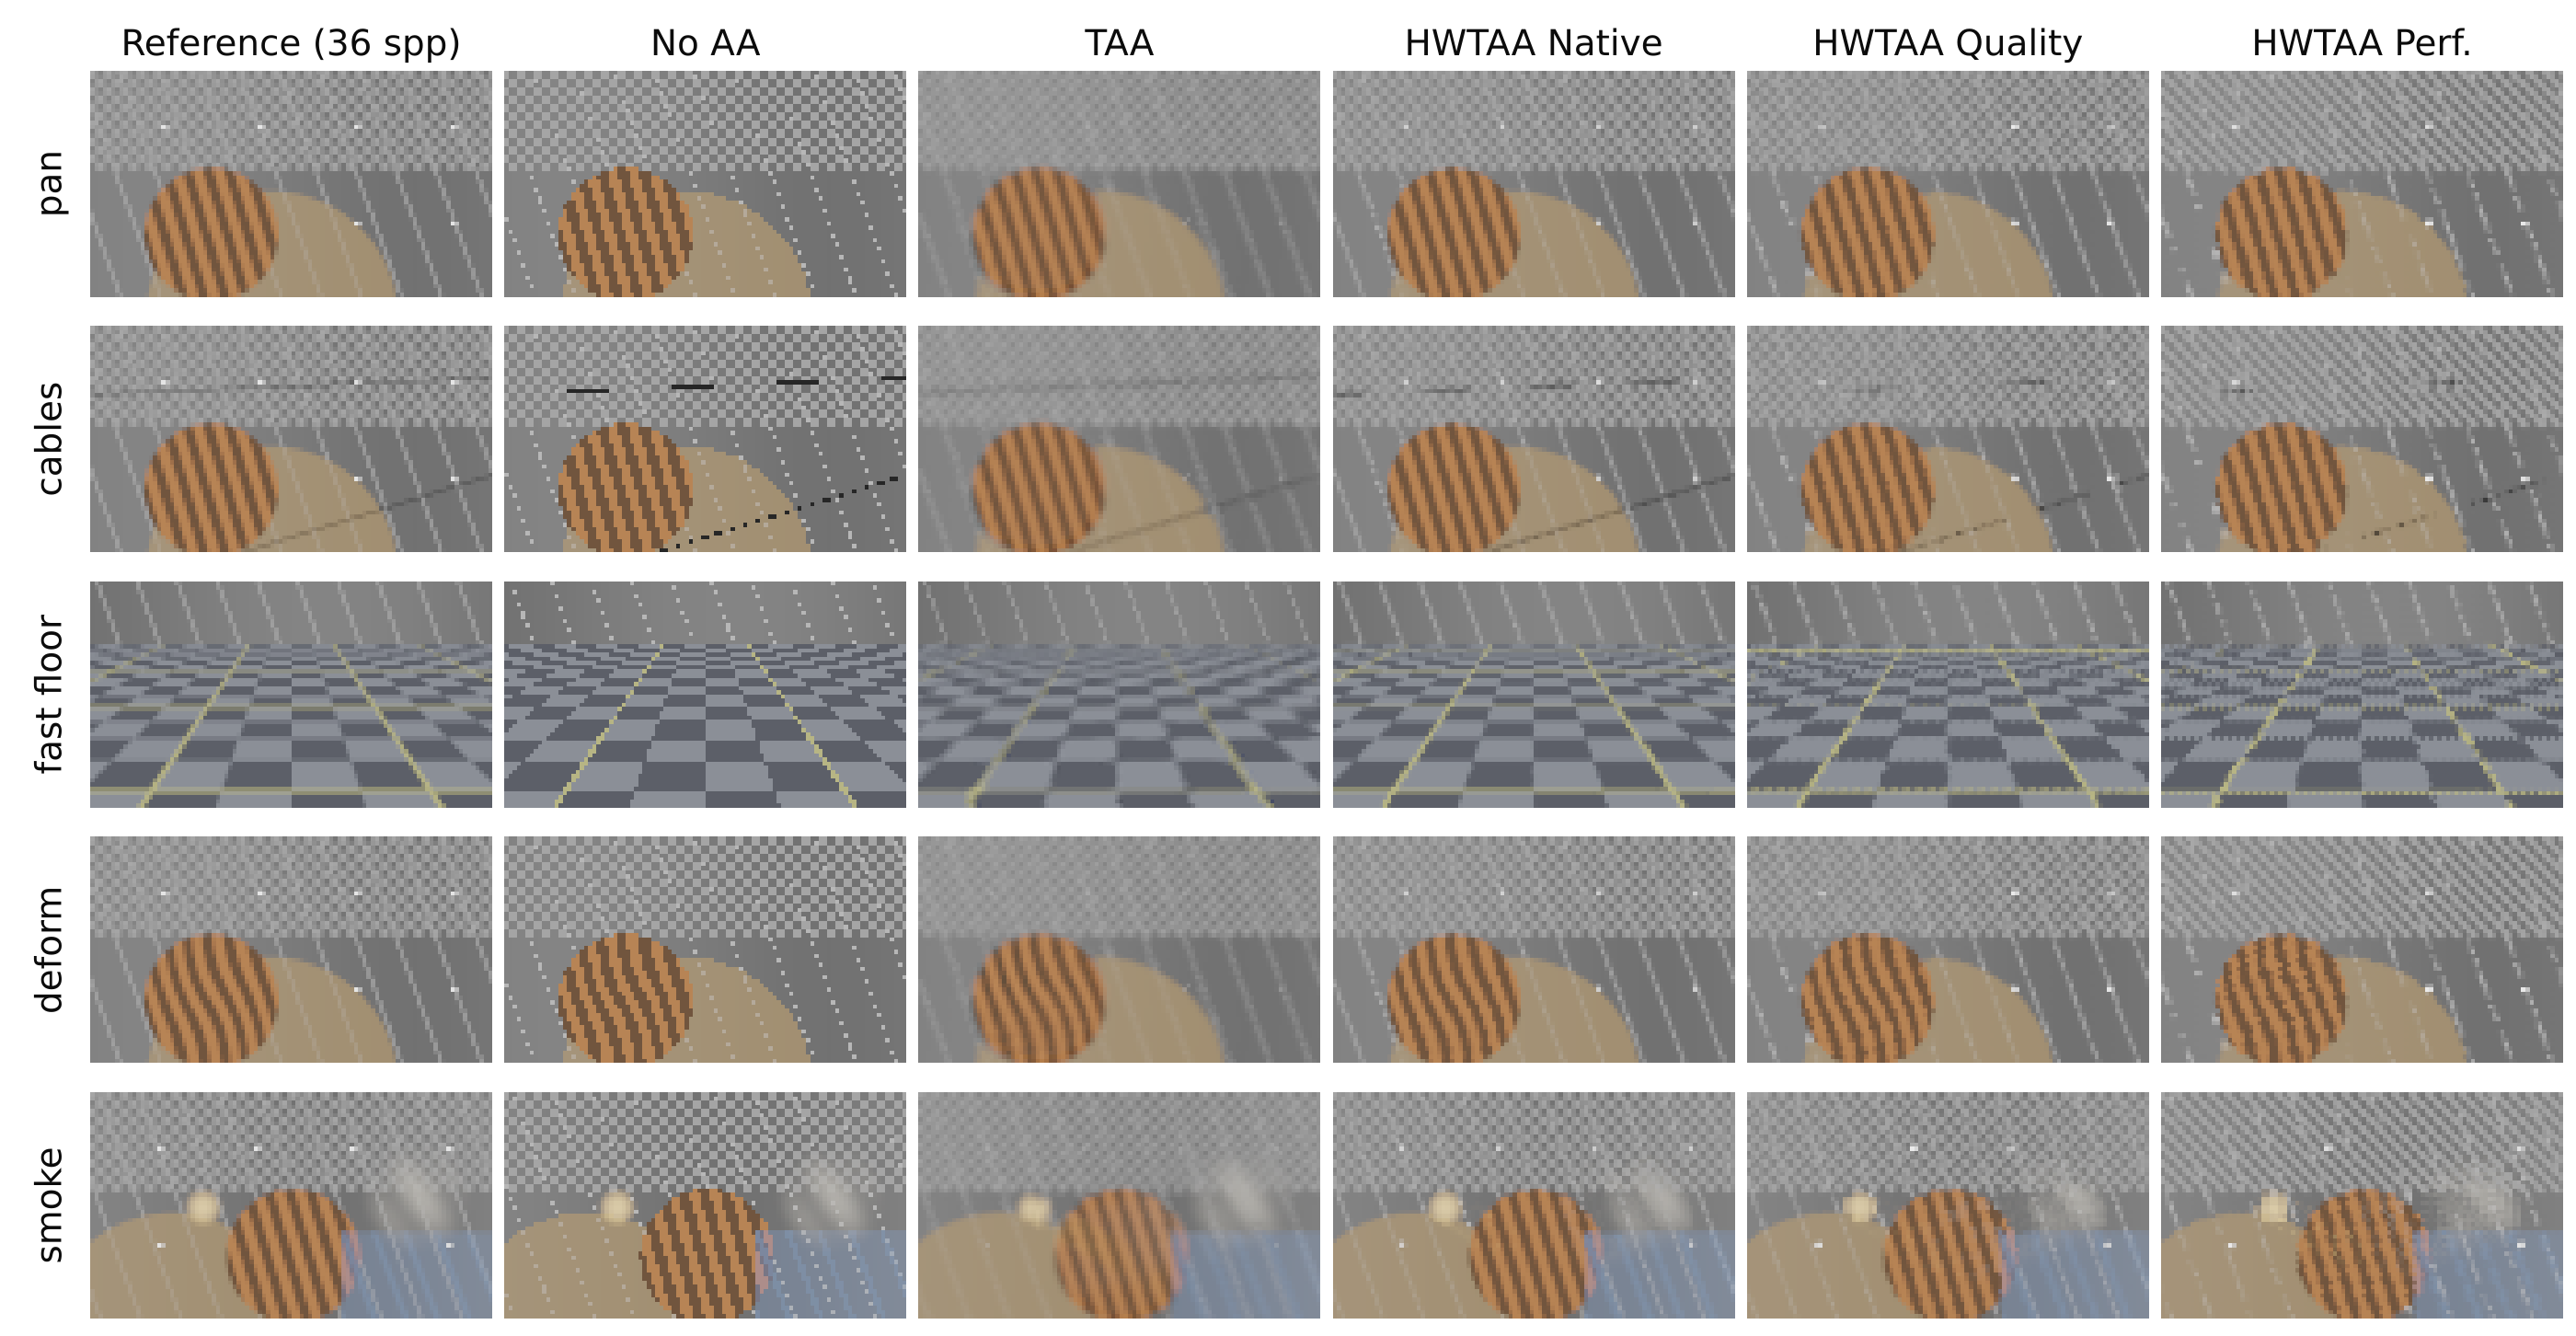
\includegraphics[width=\textwidth]{crops.png}
\caption{Frame 45 of five scenes, $96\times54$ crops shown with nearest-neighbor magnification. TAA blurs the 2-pixel checkers and the lines in motion and loses most of the cables; HWTAA Native keeps them. The upscaling modes render 44\,\% (Quality) and 25\,\% (Performance) of the pixels: cables break into dashes and the deformed disk shows its sampling pattern at Performance.}
\label{fig:crops}
\end{figure}

\Cref{fig:crops} shows the difference in motion. TAA's history, resampled every frame, has lost the checkers, the lines and most of the cables; the window, which never resamples, keeps them. At low render scales the window has too few samples for sub-pixel features: cables become dashed at Quality and Performance, and the deformed disk, whose window is 6 frames long, shows its sampling pattern.

\subsection{Window length}

\begin{figure}[t]
\centering
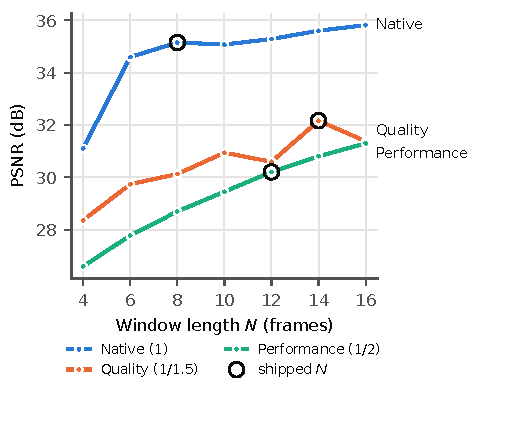
\includegraphics[width=0.62\textwidth]{window.pdf}
\caption{PSNR against the window length $N$, mean of \emph{pan}, \emph{cables} and \emph{floor}, per render scale. Circles mark the length each mode ships with. At render scale $1/1.5$ the window length is also the jitter cycle in motion, and the cycles of 12 and 16 phases cover the pixel worse than 14.}
\label{fig:window}
\end{figure}

\Cref{fig:window} shows the effect of the window length. At native resolution the gain saturates after 6 to 8 frames; 14 to 16 frames gain another 0.5 to 0.7\,dB, but each frame costs about \nMsPerFrameHd{}\,ms at 1080p for the pixels in motion. When upscaling, every frame adds samples that the output pixel lacks; at half resolution the PSNR keeps rising up to 16 frames. The shipped lengths are a cost decision.

\subsection{Disocclusion}

\begin{figure}[t]
\centering
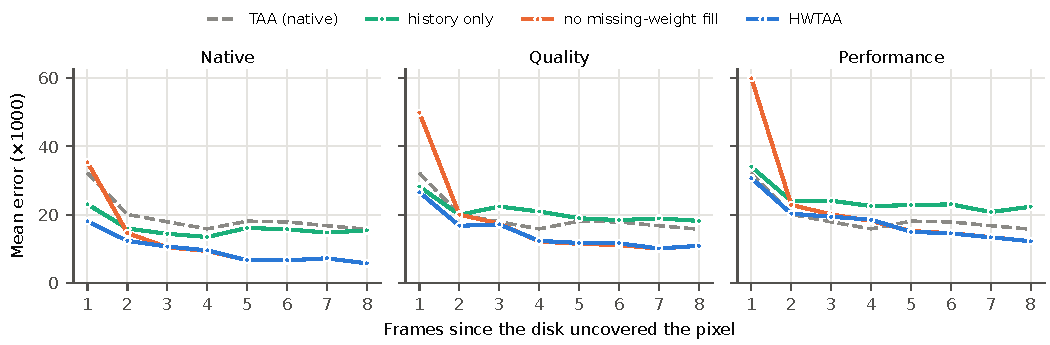
\includegraphics[width=\textwidth]{ghost.pdf}
\caption{Mean error ($\times1000$) on the pixels the moving disk of \emph{pan} uncovered, by frames since they were uncovered. Without the missing-weight fill, the window pulls the disk's edge into the first frame after uncovering; the history alone stays blurred for the following frames.}
\label{fig:ghost}
\end{figure}

\Cref{fig:ghost} follows the pixels the moving disk uncovers. In the first frame after uncovering, the window alone is worse than the history, because the uncovered surface has no past samples there and the disk's samples pull the edge; the missing-weight fill brings the error below the history's (\nGhostHwNatOne{} against \nGhostNoFillNatOne{} without fill and \nGhostHistNatOne{} for the history alone, at native resolution). From the second frame on, the window has real samples of the uncovered surface and its error is \nGhostVsHistNat\,\% lower than the history's on average at native resolution and \nGhostVsHistQ\,\% lower at Quality.

\subsection{Ablations}

\begin{table}[t]
\centering
\caption{Ablations: each variant removes one component. PSNR changes are means over the scenes the component acts on: history only, pan, cables, floor, fast floor, deform and smoke; window only, pan-idle and static; missing-weight fill, the same as history only without smoke; locks, pan-idle, static, floor and fast floor; the others, the scene of their targeted region. On every other scene of the ablation set the change is at most \nAblNoMissingFillRest{}\,dB, except for the history-only variant, which also changes pan-idle by $\nAblHistoryOnlyPausestopNat$\,dB. The last two columns give the relative change of the targeted region error or flicker.}
\label{tab:ablation}
\small\setlength{\tabcolsep}{4pt}
\begin{tabular}{lrrlrr}
\toprule
Variant & $\Delta$ Native & $\Delta$ Quality & \multicolumn{3}{c}{Targeted region} \\
\cmidrule(lr){4-6}
 & dB & dB & & Native & Quality \\
\midrule
History only (no window) & $-5.65$ & $-4.41$ & uncovered (pan) & $+50$\,\% & $+31$\,\% \\
Window only (no history) & $-0.30$ & $-0.03$ & flicker (static) & $+161$\,\% & $+147$\,\% \\
No missing-weight fill & $-0.35$ & $-0.37$ & uncovered (pan) & $+27$\,\% & $+25$\,\% \\
No luma locks & $-2.56$ & $-2.88$ & sky (fast floor) & $+25$\,\% & $+3$\,\% \\
No thin-foreground rule & $-0.22$ & $-0.16$ & cables (cables) & $+12$\,\% & $+12$\,\% \\
No window on deformed meshes & $-0.59$ & $-0.72$ & deformed disk (deform) & $+62$\,\% & $+104$\,\% \\
No reactive mask & $-2.27$ & $-1.44$ & smoke trail (smoke) & $+133$\,\% & $+140$\,\% \\
\bottomrule
\end{tabular}

\end{table}

\Cref{tab:ablation} removes one component at a time, at native resolution and in Quality mode. Without the window, the PSNR of the moving scenes changes by $\nAblHistoryOnlyNat$\,dB at native resolution and by $\nAblHistoryOnlyQ$\,dB in Quality mode: the window is the main contribution. Without the history, the PSNR barely changes on average, but on the static scene the PSNR changes by $\nAblWindowOnlyStaticNat$\,dB and the flicker by $\nAblWindowOnlyStaticNatFlicker$\,\%, because the window stops converging after $N$ frames, and the resolve costs more: on a pixel at rest the history path costs \nHistShareNat\,\% of the window path at native resolution and \nHistShareQ\,\% in Quality mode. Right after the camera stops (\emph{pan-idle}) the window alone scores $\nAblWindowOnlyPausestopNat$\,dB against the hybrid, whose history has not converged yet; we return to this in \cref{sec:limitations}. The locks are essential for thin features at rest ($\nAblNoLocksStaticNat$\,dB on \emph{static} without them). Without the reactive mask the error of the smoke's trail grows by \nAblNoReactiveTgtNatAbs\,\% at native resolution; without the window on deformed meshes the error of the deformed disk grows by \nAblNoDeformedWindowTgtNatAbs\,\% at native resolution and by \nAblNoDeformedWindowTgtQAbs\,\% in Quality mode. The thin-foreground rule and the missing-weight fill have smaller but consistent effects where they apply.

\subsection{Cost and memory}
\label{sec:cost}

\begin{table}[t]
\centering
\caption{Cost and memory. HWTAA: estimated time on an RX~590 (GTX~1060 class) with the pixels at rest and with the whole screen in motion, the worst case; memory in MB with the ring, history, locks, object identifiers and reactive mask. \textsuperscript{a}FSR~2.2: measured by AMD on an RX~590~\cite{amd2023fsr2}. \textsuperscript{b}FSR~3.1: AMD's figures for an RX~5700~XT~\cite{amd2024fsr3,amd2025fsr31manual}, a faster GPU, for reference only.}
\label{tab:cost}
\small
\begin{tabular}{llrrrrrrrr}
\toprule
 & & & \multicolumn{2}{c}{HWTAA (ms)} & \multicolumn{2}{c}{FSR (ms)} & \multicolumn{3}{c}{Memory (MB)} \\
\cmidrule(lr){4-5}\cmidrule(lr){6-7}\cmidrule(lr){8-10}
Output & Mode & $N$ & Still & Moving & 2.2\textsuperscript{a} & 3.1\textsuperscript{b} & HWTAA & 2.2 & 3.1 \\
\midrule
1080p & Native & 8 & 0.8 & 1.4 & -- & 1.7 & 189 & -- & -- \\
 & Ultra Quality & 14 & 0.7 & 2.0 & -- & -- & 188 & -- & -- \\
 & Quality & 14 & 0.6 & 2.0 & 1.3 & 1.2 & 151 & 115 & 75 \\
 & Balanced & 14 & 0.6 & 2.0 & 1.2 & -- & 127 & 105 & 65 \\
 & Performance & 12 & 0.6 & 1.8 & 1.1 & 1.0 & 95 & 101 & 61 \\
\midrule
1440p & Native & 8 & 1.4 & 2.5 & -- & 3.0 & 335 & -- & -- \\
 & Ultra Quality & 14 & 1.2 & 3.6 & -- & -- & 333 & -- & -- \\
 & Quality & 14 & 1.1 & 3.6 & 2.3 & 2.0 & 269 & 207 & 134 \\
 & Balanced & 14 & 1.1 & 3.6 & 2.1 & -- & 226 & 189 & 118 \\
 & Performance & 12 & 1.1 & 3.1 & 1.9 & 1.7 & 169 & 172 & 101 \\
\midrule
4K & Native & 8 & 3.2 & 5.5 & -- & 6.5 & 755 & -- & -- \\
 & Ultra Quality & 14 & 2.6 & 8.2 & -- & -- & 750 & -- & -- \\
 & Quality & 14 & 2.6 & 8.1 & 5.4 & 4.4 & 605 & 448 & 292 \\
 & Balanced & 14 & 2.5 & 8.0 & 4.9 & -- & 508 & 407 & 256 \\
 & Performance & 12 & 2.4 & 7.0 & 4.4 & 3.7 & 379 & 376 & 226 \\
\bottomrule
\end{tabular}

\end{table}

We had no GPU available for this work, so the cost is estimated statically. The ACO compiler reports the inverse throughput of each shader per wave on AMD Polaris; we convert it to time on an RX~590 (36 compute units at 1.545\,GHz) with a single factor that maps FSR~2.2's own shaders, compiled the same way, to AMD's measured 1.3\,ms at 1080p in Quality mode on that GPU~\cite{amd2023fsr2}. The store pass scales with the render pixels and the resolve with the output pixels; FSR~2.2's published times on the same GPU scale the same way (1.78 and 4.15 times the 1080p time at 1440p and 4K). We also floor each estimate by its memory traffic at 192\,GB/s, the bandwidth of a GTX~1060; this matters only at native resolution, where the pixel at rest moves about 73 bytes. The bench includes a script that measures both passes with GPU timer queries on real hardware.

\Cref{tab:cost} compares the estimates with FSR. At rest, HWTAA costs about half of FSR~2.2 in the upscaling modes (\nMsStillQHd{} against 1.3\,ms at 1080p Quality). With the whole screen in motion, the window's cost grows with $N$ by about \nMsPerFrameHd{}\,ms per frame at 1080p, and HWTAA costs 1.5 to 1.6 times FSR~2.2 (\nMsMovingQHd{} against 1.3\,ms at 1080p Quality, \nMsMovingQUhd{} against 5.4\,ms at 4K). At native resolution there is no FSR~2.2 mode to compare with; FSR~3.1's Native AA takes 1.7\,ms at 1080p on a faster GPU, against \nMsStillNatHd{} to \nMsMovingNatHd{}\,ms for HWTAA. Memory is dominated by the ring: in Quality mode it is 1.3 times FSR~2.2's and 2 times FSR~3.1's; in Performance mode it is close to FSR~2.2's.

\section{Limitations and future work}
\label{sec:limitations}

\paragraph{Evaluation.} The scenes are synthetic and small, and their reference is analytic. They were designed to isolate the cases that TAA handles badly, so their averages overstate the gain on typical game content, where much of the screen is at rest and both methods converge. Times are compiler estimates, not measurements; the calibration on FSR~2.2 makes them comparable with AMD's figures, but the real cost depends on the GPU, the driver and the scene. We did not measure the image quality of FSR, DLSS or other upscalers on the bench. A study on game content on real hardware, against these methods, is the natural next step.

\paragraph{Cost and memory in motion.} The window costs about \nMsPerFrameHd{}\,ms per frame of the window at 1080p for the pixels in motion, \nMsPerFrameUhd{}\,ms at 4K, which makes a full-screen pan at 4K more expensive than FSR. Its ring takes 1.3 to 2 times FSR's memory. Both are tunable through the window length and the memory budget, at about 0.3\,dB per frame of window when upscaling.

\paragraph{Low render scales.} At a quarter of the pixels a 12-frame window holds three samples per output pixel; fast motion, strong per-sample noise and zooming out then favor TAA's longer accumulation.

\paragraph{Pixels that stop.} For a few frames after a pixel stops, its history has not converged while the window still holds $N$ valid samples (\emph{pan-idle} in \cref{tab:ablation}). Keeping the window until the history's confidence reaches the window's weight would remove this gap.

\paragraph{Engine requirements.} The method needs stable object keys, object motion of the past $N$ frames and a velocity buffer for deformed meshes, which a game engine has but a post-process injected into an arbitrary application does not. Deformed meshes extrapolate their past positions from the current velocity, which limits their window to a few frames.

\section{Conclusion}

TAA summarizes the past in one image and pays for it every frame a pixel moves. HWTAA keeps the past samples themselves for a short window, moves each of them exactly once to the current frame and decides their visibility by identity, and keeps the recursive history only where it is at its best, on pixels at rest. On our scenes this improves a production-grade TAA by \nGainAllNat{}\,dB at native resolution and by \nGainAllQ{}\,dB while upscaling from 44\,\% of the pixels, and it keeps cables, lines and fine texture sharp in motion. The price is memory for the ring and a cost in motion that grows with the window, both of which an application can tune.

\section*{Use of AI tools}
The method was developed by the author with the assistance of Claude (Anthropic), an AI model, used as a programming and research assistant: it implemented and measured variants under the author's direction, built the evaluation bench and helped draft this manuscript. The author directed the work, made the design decisions and is responsible for the content. The AI tool is not listed as an author.

\section*{Code and data}
The shaders and the evaluation bench, with the scripts that produce every table and figure, are in the same repository as this paper, under the GNU General Public License version 2 or later, like the UPBGE engine.

\bibliographystyle{unsrtnat}
\bibliography{../refs}

\end{document}
